% -----------------------------------------------
% Template for ISMIR Papers
% 2025 version, based on previous ISMIR templates

% Requirements :
% * 6+n page length maximum
% * 10MB maximum file size
% * Copyright note must appear in the bottom left corner of first page
% * Clearer statement about citing own work in anonymized submission
% (see conference website for additional details)
% -----------------------------------------------

\documentclass{article}
\usepackage[T1]{fontenc}
\usepackage[utf8]{inputenc}
\usepackage{ismir} % Remove the "submission" option for camera-ready version
\usepackage{amsmath,cite,url}
\usepackage{graphicx}
\usepackage{color}
\usepackage{booktabs}
\usepackage{placeins}
\usepackage{amssymb}% http://ctan.org/pkg/amssymb
\usepackage{pifont}% http://ctan.org/pkg/pifont

% \crefformat{footnote}{#2\footnotemark[#1]#3}

\usepackage{algorithm} % Added
\usepackage{algpseudocode} % Added
\usepackage{gensymb} % Added
\usepackage{siunitx} % Added
\usepackage{multirow} % Added
\usepackage{siunitx} % Added
\sisetup{input-symbols = ()} % Added
\usepackage{kotex}
\newcommand{\cmark}{\ding{51}}%
\newcommand{\xmark}{\ding{55}}%
\usepackage{microtype} % Added
\usepackage{paralist} % Added
\usepackage{float} % added

\newcommand{\alex}[1]{\textcolor{blue}{#1}}%
\newcommand{\jh}[1]{\textcolor{red}{#1}}

% Title. Please use IEEE-compliant title case when specifying the title here,
% as it has implications for the copyright notice
% ------
\title{PianoVAM: A Multimodal Piano Performance Dataset}
% 타이틀 정하기가 가장 어려운 것 같아요... (용현) ㅋ(준형) 인정합니다(기락) 

% Note: Please do NOT use \thanks or a \footnote in any of the author markup

% Single address
% To use with only one author or several with the same address
% ---------------
% \oneauthor
%   {Anonymous Authors}
%   {Anonymous Affiliations\\\texttt{anonymous@ismir.net}}

% Two addresses
% --------------
%\twoauthors
%   {First author} {School \\ Department}
%   {Second author} {Company \\ Address}

% Three addresses
% --------------
% \threeauthors
%   {First Author} {Affiliation 1 \\ \texttt{author1@ismir.edu}}
%   {Second Author} {Affiliation 2 \\ \texttt{author2@ismir.edu}}
%   {Third Author} {Affiliation 3 \\ \texttt{author3@ismir.edu}}

% Four or more addresses
% OR alternative format for large number of co-authors
% ------------
\multauthor
  {Yonghyun Kim$^\flat$ \hspace{1cm} Junhyung Park$^\natural$ \hspace{1cm} Joonhyung Bae$^\sharp$ \hspace{1cm} Kirak Kim$^\sharp$}
  {{\bf Taegyun Kwon$^\sharp$ \hspace{1cm} Alexander Lerch$^\flat$ \hspace{1cm} Juhan Nam$^\sharp$}\\
  $^\flat$ Music Informatics Group, Georgia Institute of Technology, USA\\
  $^\natural$ Department of Mathematical Sciences, KAIST, South Korea\\
  $^\sharp$ Graduate School of Culture Technology, KAIST, South Korea\\
  {\tt\small \{yonghyun.kim,alexander.lerch\}@gatech.edu,\\
  \tt\small \{tonyishappy,jh.bae,kirak,ilcobo2,juhan.nam\}@kaist.ac.kr}
  }

% For the author list in the Creative Common license, please enter author names.
% Please abbreviate the first names of authors and add 'and' between the second to last and last authors.
\def\authorname{Y. Kim, J. Park, J. Bae, T. Kwon, K. Kim, A. Lerch and J. Nam}

% Optional: To use hyperref, uncomment the following.
\usepackage[bookmarks=false,pdfauthor={\authorname},pdfsubject={\pdfsubject},hidelinks]{hyperref}

% \usepackage{cleveref} % Added for mutliple footnote

% Mind the bookmarks=false option; bookmarks are incompatible with ismir.sty.

\sloppy % please retain sloppy command for improved formatting

\begin{document}

\maketitle

\begin{abstract}

The multimodal nature of music performance has driven increasing interest in data beyond the audio domain within the music information retrieval (MIR) community.
%The convergence of music performance research and machine learning has created a growing demand for multimodal datasets integrating audio, video, and symbolic data. 
This paper introduces PianoVAM, a comprehensive piano performance dataset that includes videos, audio, MIDI, hand landmarks, fingering labels, and rich metadata.
The dataset was recorded using a Disklavier piano, capturing audio and MIDI from amateur pianists during their daily practice sessions, alongside synchronized top-view videos in realistic and varied performance conditions. 
%The metadata includes piece and performer information and keyboard corner coordinates.
Hand landmarks and fingering labels were extracted using a pretrained hand pose estimation model and a semi-automated fingering annotation algorithm.
%Additionally, the dataset incorporates fingering labels primarily generated by a MediaPipe-based heuristic algorithm, with human annotations added for undetected cases. 
We discuss the challenges encountered during data collection and the alignment process across different modalities. Additionally, we describe our fingering annotation method based on hand landmarks extracted from videos.
%This paper outlines the challenges encountered during data collection and preprocessing, along with the solutions devised.
Finally, we present experimental results on both audio-only and audio-visual piano transcription using the PianoVAM dataset for benchmarking purposes and discuss other potential applications. 

\end{abstract}

\begin{figure}
    \centering
    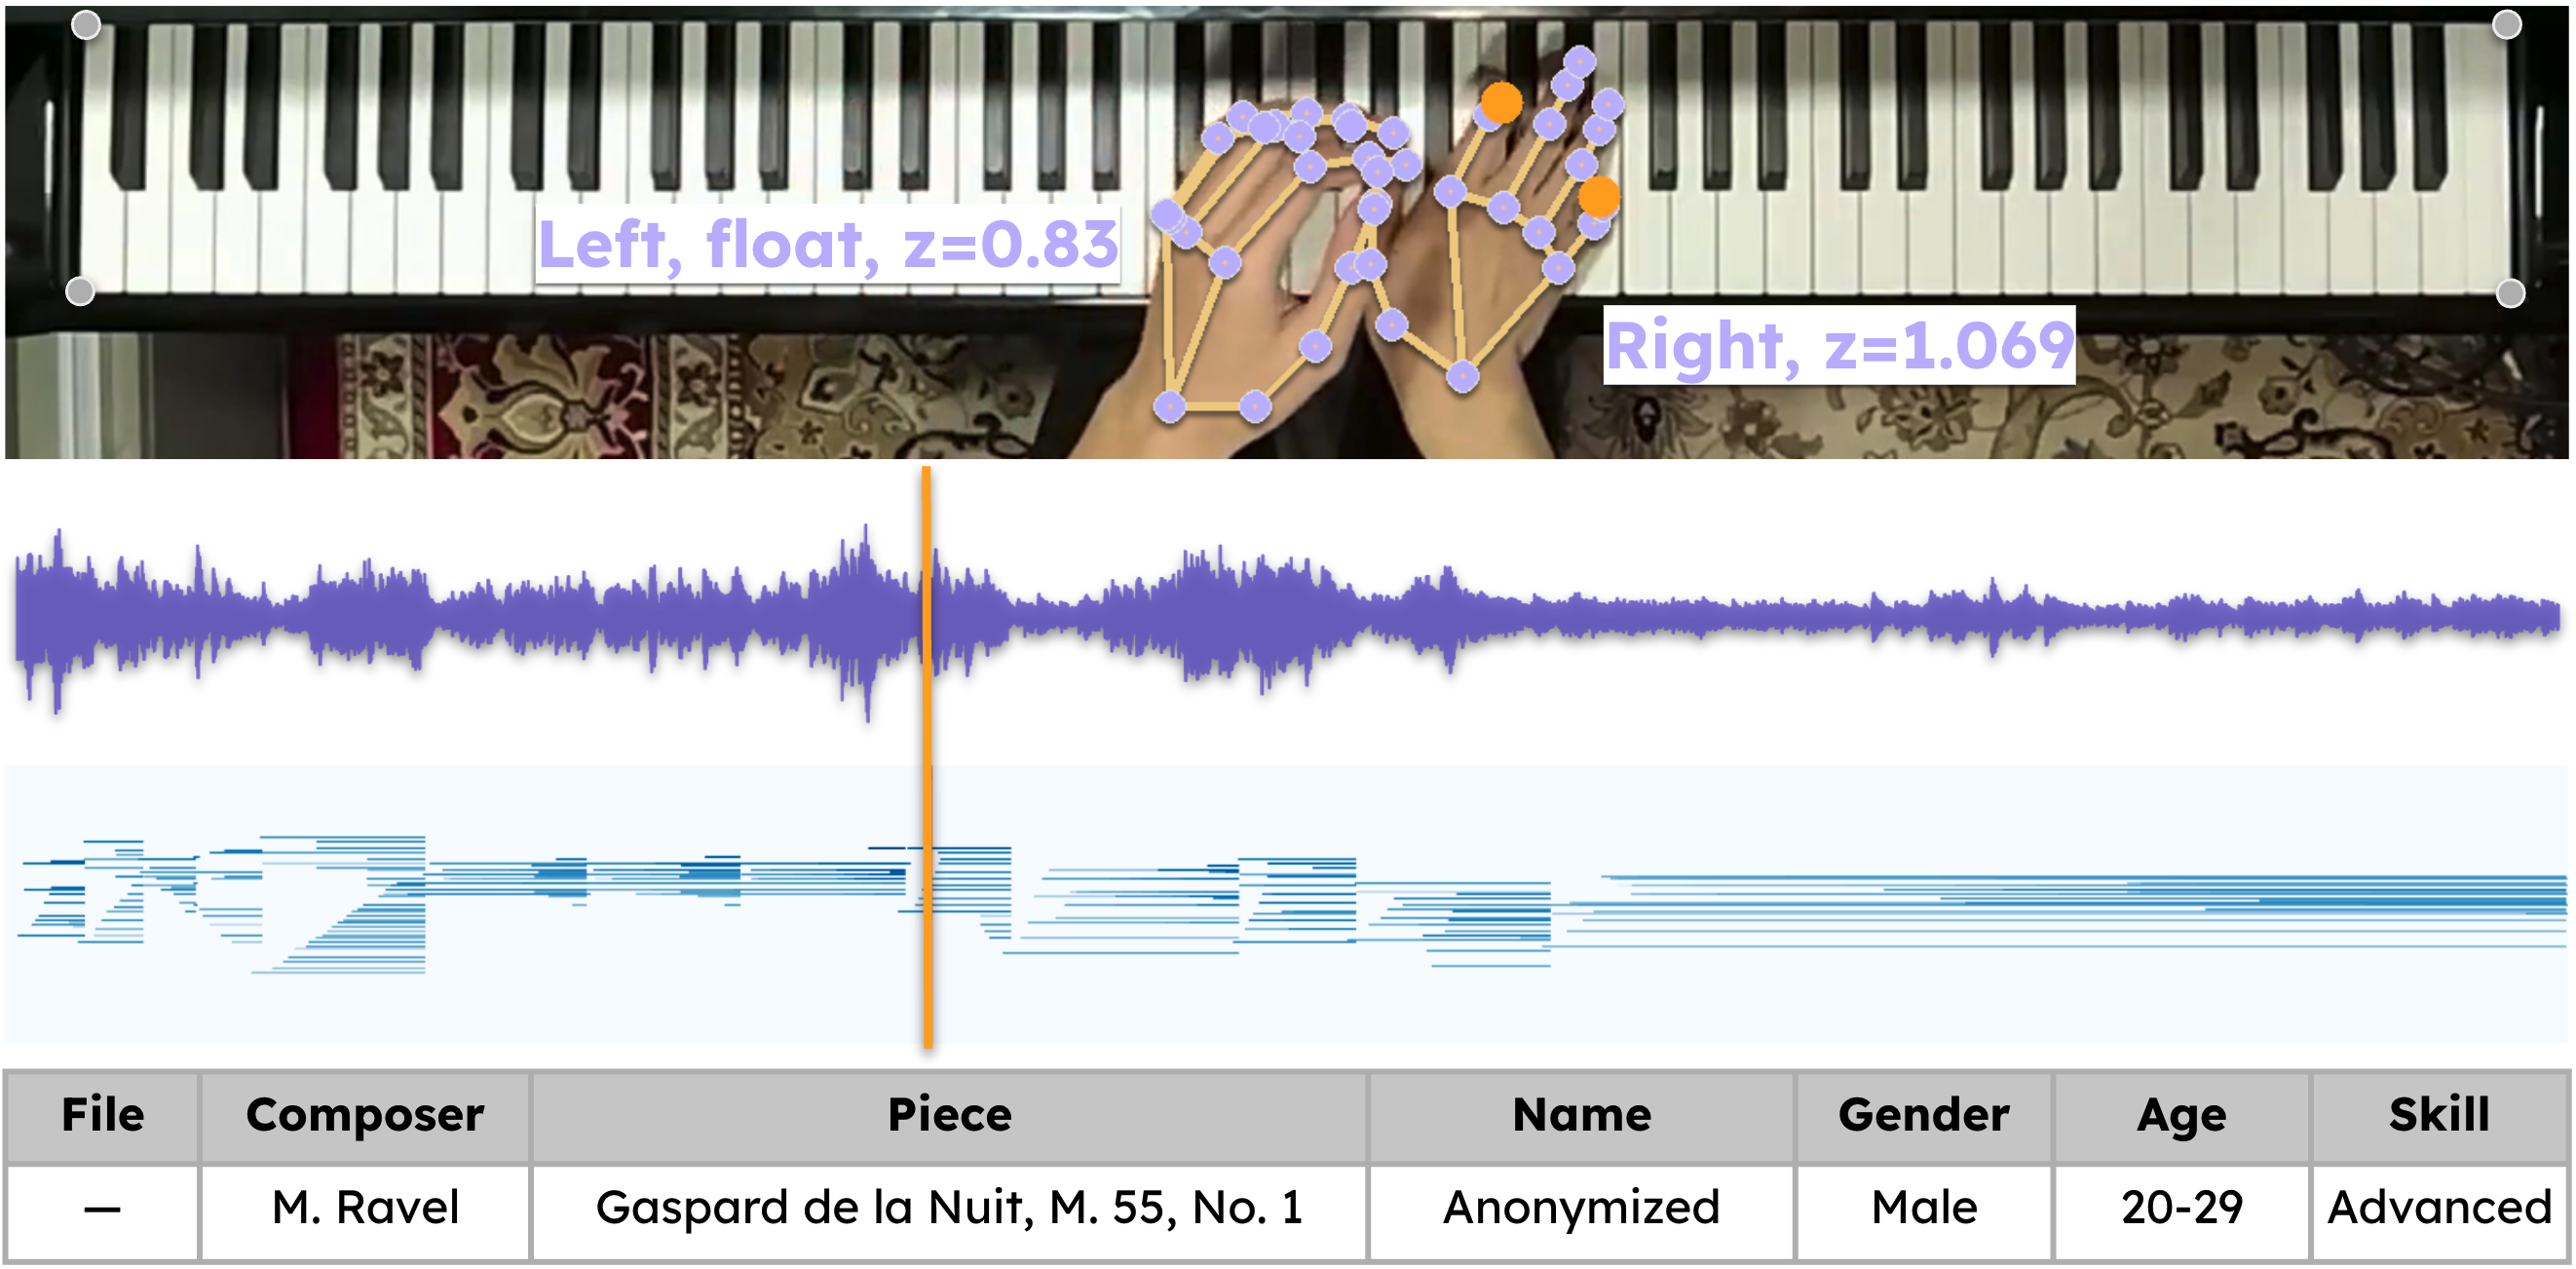
\includegraphics[width=1\linewidth]{Images/teaser_image.png}
    \caption{The PianoVAM Dataset: Synchronized video, audio, MIDI with fingering, hand landmarks, and metadata.}
    \label{fig:overview}
\vspace{-5mm}    
\end{figure}

\section{Introduction}\label{sec:introduction}

%to enhance the extraction of musical information by leveraging multiple modalities \cite{IEEE19Duan, TMM18Li, MMSP20Montesinos, arXiv24Yoo, ICASSPW23Li}. 

Music performance is inherently multimodal, involving not only audio but also motion, posture, and other visual elements as part of the expressive sound creation process \cite{PPR09Bergeron, MusicPercep12Platz}. In the field of Music Information Retrieval (MIR), there has been growing interest in collecting multimodal performance data to enhance the extraction of musical information by leveraging multiple modalities \cite{TMM18Li, IEEE19Duan}. Such multimodal data — particularly audiovisual data — have been utilized in various MIR tasks across diverse musical genres. Examples include automatic MIDI transcription of solo piano performances \cite{ICASSP20Koepke, ICASSPW23Li}, vibrato analysis of polyphonic string music \cite{SMC17Li}, singing voice separation \cite{BMVC21Montesinos}, and melodic motif identification in Indian vocal performances \cite{TISMIR24Nadkarni}. In these tasks, visual information from performer videos has been shown to improve model robustness by providing additional musical cues. This paper focuses on the multimodal data collection of solo piano performances to improve transcription and explore other potential applications.  

\begin{table*}[t]
    \centering
    \small
    \begin{tabular}{lcccccc}
        \toprule
        \textbf{Dataset}  & \textbf{Size (hrs)} & \textbf{Video} & \textbf{Audio} & \textbf{Audio Type} & \textbf{MIDI} & \textbf{Fingering} \\
        \midrule
        MAESTROv3 \cite{ICLR19Hawthorne}  & 198.7  & \xmark  & {44.1--48}\si{kHz}, Stereo & Real  & \cmark & \xmark \\
        MAPS (MUS subset) \cite{Emiya2010}     & 18.6  & \xmark     & 44.1\si{kHz}, Stereo & Synth. \& Real & \cmark & \xmark \\
        OMAPS2 \cite{ICASSPW23Li}   & 6.7  & 1080p/30fps & 44.1\si{kHz}, Mono & Real & $\triangle$ (.TXT)  & \xmark \\
        PianoYT \cite{ICASSP20Koepke}  & $\sim$20  & Varies  & Varies (YouTube) & Varies (YouTube) & $\triangle$ (Pseudo) & \xmark \\
        PianoVAM (Ours) & 21.0 & 1080p/60fps & 44.1\si{kHz}, Mono & Real  & \cmark & $\triangle$ (Pseudo) \\
        \bottomrule
    \end{tabular}
\vspace{-2mm}    
    \label{tab:piano_datasets}
\caption{Comparison of Piano Transcription Datasets.}
\end{table*}
\begin{table*}[!h]
    \centering

    \small
    \begin{tabular}{lcccccc}
        \toprule
        \textbf{Dataset}  & \textbf{Total notes} & \textbf{\# of pieces} & \textbf{Labeled ratio (\%)} & \textbf{Data type} & \textbf{Reliability} & \textbf{Annotation} \\
        \midrule
        PIG \cite{InfoSci20Nakamura} & 100,044 & 309 & 100 & MIDI \& Score (.PDF) & By pianists & Manual \\
        ThumbSet \cite{MM22Ramoneda} & -- & 2,523 & 52 & MusicXML & By miscellaneous & Manual \\
        PianoVAM (Ours) & 1,050,966 & 106 & 100 & Multimodal & $\sim$ 0.95 & Semi-Auto \\
        \bottomrule
    \end{tabular}
\vspace{-2mm}    
\caption{Comparison of Piano Fingering Datasets.}
    \label{tab:fingering-datasets}
\vspace{-2mm}    
\end{table*}

Piano transcription, which converts audio recordings into symbolic representations like MIDI or sheet music, is a well-established MIR task that has made significant progress through large-scale, clean audio-MIDI datasets such as MAESTRO \cite{ISMIR18Hawthorne} and carefully designed deep learning models \cite{TASLP21Kong, ISMIR22Wei}. As benchmarking performance on the MAESTRO dataset approaches its ceiling \cite{ISMIR24Yan}, new challenges have emerged in piano transcription. One major challenge is achieving acoustic robustness to ensure reliable transcription from real-world piano performance recordings, which often feature diverse piano timbres, reverberations, or other interfering noise sources. While data augmentation has been a common technique to address this issue \cite{ICLR19Hawthorne, Edwards2024}, leveraging visual data from performance videos has recently emerged as an alternative research direction \cite{CJE15Wan, DAFx21Wang, ICASSPW23Li, TASLP24Li}. Another key challenge is capturing richer performance information beyond a single MIDI track, such as left-right hand separation, piano fingering, and other playing details \cite{InfoSci20Nakamura, MM22Ramoneda}. Achieving this requires capturing visual-domain data, such as performer motion or keyboard-view videos, and synchronizing them with audio and MIDI data. However, collecting such multimodal data is both costly, requiring a dedicated data acquisition system, and time-consuming, as it depends on the availability of prepared piano players. 

This paper introduces PianoVAM, a comprehensive piano performance dataset that includes videos, audio, MIDI, hand landmarks, fingering labels, and rich metadata. An overview of PianoVAM is presented in Figure \ref{fig:overview}. The dataset was collected from amateur pianists during their daily practice sessions on a Disklavier piano, with synchronized top-view videos captured in realistic and varied performance conditions. We extracted hand landmarks and generated fingering pseudo-labels using a pretrained hand pose estimation model combined with a semi-automated fingering detection algorithm.  We describe the challenges faced during data collection and the alignment of multiple modalities. Furthermore, we detail our fingering annotation method, which utilizes hand landmarks extracted from the videos. Lastly, we present experimental results on both audio-only and audio-visual piano transcription using the PianoVAM dataset for benchmarking, along with a discussion of its potential applications. PianoVAM is available for download from the GitHub page\footnote{https://yonghyunk1m.github.io/PianoVAM\label{github-link}} under the CC BY-NC 4.0 license.


\section{Related Work}
% Revised (Camera-ready)
\subsection{Audio-Visual Datasets}
The emergence of audio-visual datasets represents a promising frontier in MIR, unlocking new research possibilities by providing visual information that complements audio signals. The URMP dataset \cite{TMM18Li} offers synchronized audio, video, and MIDI recordings of multi-instrument classical performances, supporting multimodal analysis of ensemble music such as audio-visual source association via vibrato modeling \cite{SMC17Li}. The Acappella dataset \cite{BMVC21Montesinos} contains solo acappella videos, enabling audio-visual singing voice separation with fine-grained control over visual and acoustic conditions. \cite{TISMIR24Nadkarni} presents an audiovisual dataset of Hindustani vocal performances annotated with melodic motifs and stable notes, enabling gesture-based music analysis and raga classification through movement-melody correspondence.

\subsection{Piano Transcription Datasets}
Table \ref{tab:piano_datasets} compares existing piano performance datasets with PianoVAM. MAESTRO \cite{ICLR19Hawthorne} includes high-quality audio and MIDI recorded from proficient pianists on Disklavier pianos but lacks top-view videos. MAPS \cite{Emiya2010} provides audio and MIDI from actual performances (MUS subset), though a significant portion (210 out of 270 recordings) is synthesized. OMAPS2 \cite{ICASSPW23Li} and PianoYT \cite{ICASSP20Koepke} incorporate video data but offer limited MIDI annotations: OMAPS2 provides MIDI-like labels, while PianoYT uses pseudo-MIDI annotations transcribed with the Onsets and Frames model \cite{ISMIR18Hawthorne}. In contrast, PianoVAM offers the most comprehensive multimodal dataset, including real performance audio, synchronized MIDI, top-view videos, and fingering pseudo-labels, although its total duration is limited.

\subsection{Fingering Datasets}
Table \ref{tab:fingering-datasets} compares existing piano fingering datasets with PianoVAM. PIG \cite{InfoSci20Nakamura} incorporates fingering and MIDI information of sections of several pieces played by professional pianists, which also provides different fingerings for the same piece by various pianists. In \cite{MM22Ramoneda}, they tried to annotate fingering of the complete piece from partially annotated MusicXML files with the support of ThumbSet dataset, which crowdsourced fingering information of numerous pieces from MuseScore\footnote{\href{https://musescore.com}{https://musescore.com} (Last accessed: June 28, 2025)}, an online piano score website, but the source of fingering annotation is not clear. To address this, we have incorporated reliable fingering annotations into the PianoVAM dataset. These annotations are created by applying our fingering detection algorithm to top-view video data synced with MIDI and then manually annotating incomplete labels to improve reliability. % Revised (Camera-ready)


\section{Dataset Acquisition \& Preprocessing}\label{sec:dataset-acquisition-preprocessing}

\subsection{Acquisition}
We developed a data acquisition system to streamline the unsupervised recording of video, audio, MIDI, and associated metadata, such as performer and piece details.  
 
\begin{figure*}
    \centering
    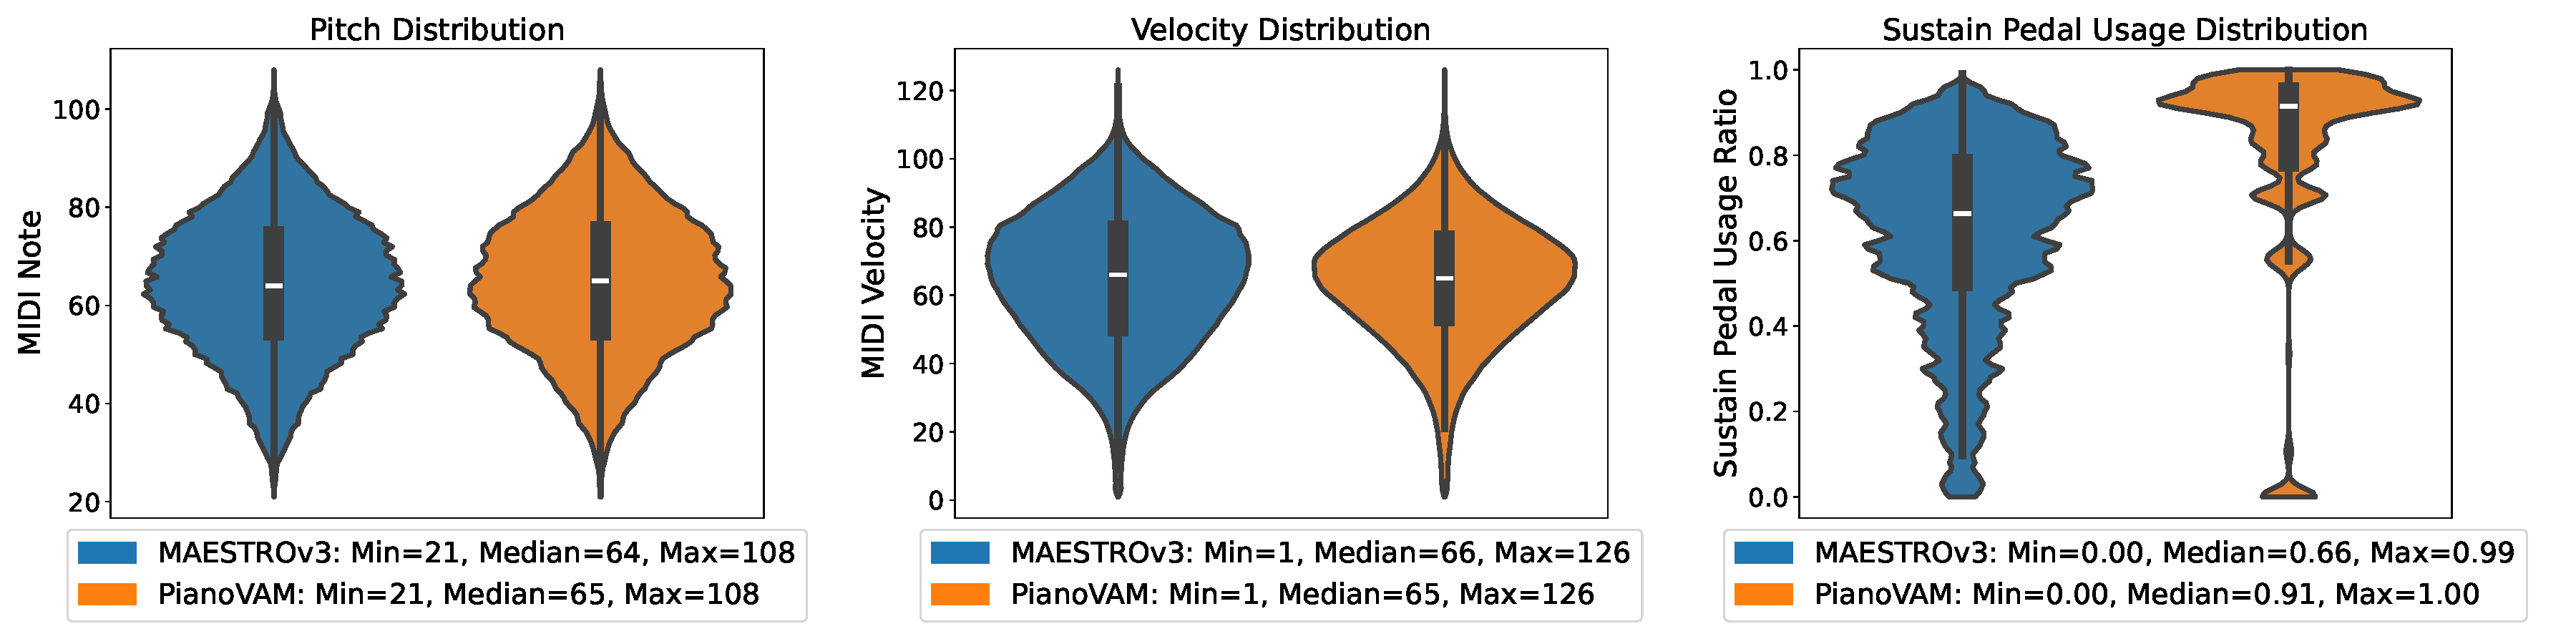
\includegraphics[width=1\linewidth]{Images/combined_violinplot.pdf}
    \vspace{-7mm}    
    \caption{Distributional comparison of pitch, velocity, and pedal usage between MAESTROv3 and PianoVAM.}
    \vspace{-3mm} 
    \label{fig:combined-violinplot}
\end{figure*}


\subsubsection{Acquisition Workflow}
The acquisition workflow comprises the following steps. First, new users register by providing basic personal details and receive unique QR codes for identification and recording control. A single interface launch initializes the required software — OBS Studio for video and audio, and Logic Pro for audio and MIDI. Before recording, users input performance details and display their profile QR code to a top-view camera to begin capturing. When the performance concludes, presenting a stop QR code ends the recording.


\subsubsection{Hardware Setup} 
% A PC runs the control script along with OBS Studio and Logic Pro. A webcam mounted overhead provides the video feed, and a microphone records audio. Logic Pro captures the MIDI output from a Disklavier piano.
% A common audio signal captured by OBS Studio and Logic Pro was used to correct for recording latency.
The data acquisition process was managed by a control script on a PC. An overhead-mounted webcam captured the video, while a dedicated microphone and a Disklavier piano provided the audio and MIDI signals, respectively. OBS Studio recorded the audio-video stream, and Logic Pro concurrently recorded the audio-MIDI stream. A common audio signal captured by both systems provided a reference for an global time alignment to correct for recording latency. % Revised (Camera-ready)

\subsection{Preprocessing}
\subsubsection{Alignment}\label{subsubsec:alignment}
%https://docs.google.com/document/d/1G1aIxIEiFI9kxwOgP_GDq4pADkeToc136394PAb-5-I/edit?usp=sharing

The time alignment of audio and MIDI data was further refined using the fine alignment technique used for the MAESTRO dataset \cite{ICLR19Hawthorne}. 
Specifically, we down-mixed the recorded audio to mono and resampled it at {22.05}\si{kHz}. 
We then synthesized the provided MIDI data into an audio signal at the same sampling rate using FluidSynth with a SoundFont sampled from Disklavier Pro recordings\footnote{\href{https://freepats.zenvoid.org/Piano/YDP-GrandPiano/YDP-GrandPiano-SF2-20160804.tar.bz2}{https://freepats.zenvoid.org/Piano/YDP-GrandPiano/YDP-GrandPiano-SF2-20160804.tar.bz2} (Last accessed: June 28, 2025)\label{soundfont}}, since we could not access the original Disklavier7 SoundFont used in the MAESTRO dataset.
A Constant-Q Transform was extracted from both audio signals using a hop length of 64 samples ($\sim$3\si{ms} resolution). Finally, we applied Dynamic Time Warping within a Sakoe-Chiba band of $\pm2.5$\si{s} to correct any remaining temporal discrepancies, such as small constant offsets or jitter.


\subsubsection{Audio Loudness Normalization} 
Recordings were collected over a six-month period in a shared studio, with a notable gap between May and August. This interruption may have introduced inconsistencies in loudness due to variations in recording conditions, such as gain settings or microphone placement. To mitigate potential mismatches between loudness and MIDI velocity across the dataset, we applied a loudness normalization procedure. First, the collected MIDI data were synthesized using \textit{FluidSynth} with a Disklavier-sampled SoundFont\footref{soundfont}. The integrated loudness of each synthesized audio file was measured using the \textit{pyloudnorm} package\cite{steinmetz2021pyloudnorm}. We then computed the average loudness across all rendered files and defined $-$23~\si{LUFS} as the desired global average. A uniform gain offset was calculated based on the difference between the measured average and this target. This offset was added to each file's measured loudness, resulting in a new target loudness for normalization. Each real PianoVAM audio recording was then normalized to match its corresponding target. This process enhanced loudness-velocity consistency while preserving the natural dynamic range of the performances.

\section{Dataset Statistics}\label{sec:dataset-statistics}

The dataset contains 106 solo piano recordings from 10 amateur performers, totaling approximately 21 hours. The repertoire is stylistically diverse, spanning works from 38 composers from the Baroque to modern eras (e.g., Bach, Chopin, Kapustin, Joe Hisaishi) and includes several improvisations. Performers' self-reported skill levels are advanced (70 recordings), intermediate (26), and beginner (10). Although the recording system allowed performers to choose between two performance types—Performance and DailyPractice—all recordings were self-labeled as DailyPractice, indicating the dataset primarily captures informal practice sessions where strict adherence to a score may not always be present. % Revised (Camera-ready) 

To investigate differences in expressive characteristics across datasets, we conducted a brief comparative analysis of MIDI-related distributions between MAESTROv3 and PianoVAM. Specifically, we examined three aspects displayed in \figref{fig:combined-violinplot}: 
\begin{inparaenum}[(i)]
    \item the distribution of pitch (MIDI note numbers) in the datasets, 
    \item the distribution of velocity (MIDI velocity values) in the datasets, and 
    \item the distribution of sustain pedal usage on a per-file basis.
\end{inparaenum}
We computed Cohen's \textit{d} for each musical feature to assess the practical significance of inter-dataset differences.  Pitch (\textit{d} = 0.0446) and velocity (\textit{d} = -0.0379) exhibited negligible differences between datasets. However, pedal usage revealed a large effect size (\textit{d} = 0.870), indicating a substantially higher use of the sustain pedal in PianoVAM compared to MAESTROv3. We speculate this difference stems from an interplay between a pedal-demanding Romantic/Impressionist repertoire, the generous pedaling tendencies of amateur performers in practice, and a less reverberant studio environment that encourages compensation. % Newly Added (Camera-ready)
 
%이는 곡 레퍼토리적 이유와 실제 연주 환경 양측이 모두 영향을 준 것으로 추정할 수 있습니다. 먼저, 연주된 곡에서 낭만주의·인상주의 작품군이 많다는 점}에서 음색의 풍부함과 긴 레가토 표현을 위해 페달을 빈번히 사용하게 되고, 실제 곡 난이도나 음역이 넓은 협주곡·판타지 등이 많다는 점 또한 페달 의존도를 높이는 원인이 됩니다. 동시에 아마추어 연주자들이 연습 과정을 녹음했다는 상황적 특성도 작용할 수 있는데, 곡 해석이나 테크닉 측면에서 페달을 좀 더 “길게” 혹은 “자주” 밟아 울림을 유지하려는 경향, 나아가 녹음 환경에서 음색을 풍부하게 만들려는 ‘과다한 페달링’이 발생할 여지가 크기 때문입니다.

% 페달의 사용이 음원에서의 울림정도와 관련이 있지만, 레코딩 환경 역시 중요. Blind RT60\cite{ICASSP14Dumortier}에서 제공하는 RT60을 각 데이터별로 분석을 해보았다. (The RT60 is defined as the time required for sound to decay by 60 dB once the source has been switched off.)
% % (Mar 26 22:13; Ongoing for Getting the Result)
% 일단 preliminary result로는 MAESTRO가 실제 concert hall에서 녹취된 음원이어서 Studio에서 녹취된 우리 데이터셋보다 울림이 크다. 

\section{Annotation of Fingering Labels}\label{sec:fingering_detection}
To generate fingering annotations, we developed the hybrid algorithm shown in Figure \ref{fig:fingering_diagram}. The algorithm first processes performance videos to map hand landmarks to potential finger candidates for each MIDI note. For notes with a single, unambiguous candidate, the fingering is determined automatically, achieving a precision of $\sim$95\% (cf. Table \ref{tab:fingering_results}). In ambiguous cases with multiple candidates (affecting $\sim$20\% of notes), a custom GUI prompts a human annotator to make the final selection. This approach ensures complete and accurate fingering annotations for the entire dataset.

% (Original) This section presents a semi-automated fingering annotation algorithm. Our automated fingering detection algorithm, whose pipeline is described in Figure \ref{fig:fingering_diagram}, extracted skeletal hand coordinates from performance videos and mapped them to the corresponding MIDI notes, achieving a precision of $\sim$95\%. However, the algorithm missed $\sim$\ 20\% of MIDI notes showing difficulties in handling complex playing techniques and ambiguous finger positions in videos. To address these gaps, we developed an efficient GUI-based fingering annotation tool, allowing human annotators to supplement missing fingering labels. By combining the results of the automated algorithm with manual corrections, we provide complete fingering annotations for all MIDI notes in the PianoVAM dataset.

\subsection{Inputs \& Outputs}
The inputs are video, MIDI, keyboard corner locations and lens distortion coefficients in the first frame for each video, which can also be set manually by the GUI-based annotation tool.
%Note that the input data needs a few pre-processing to apply our algorithm to other multimodal datasets.
The outputs are fingering information, and a separate MIDI file pair for each hand.


\subsection{Method}
% 
\begin{figure}[!t]
    \centering
    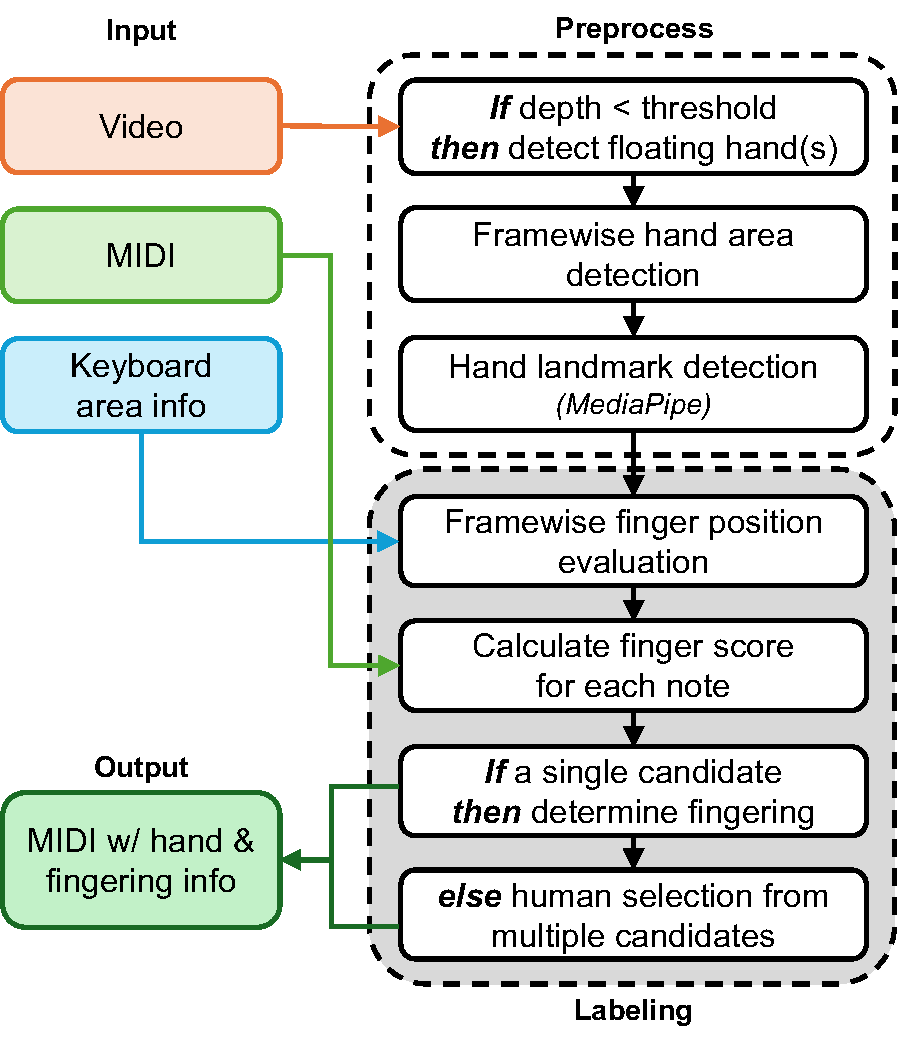
\includegraphics[width=0.9\linewidth]{Images/fingering_detection3.pdf}\hspace*{0cm}
    \caption{Flowchart of the fingering detection algorithm.}
    \label{fig:fingering_diagram}
\end{figure}

Our algorithm suggests candidates of fingers that are likely to play each note in the MIDI file. First, hand landmark information is extracted from the input video frame with MediaPipe Hands~\cite{arXiv20Zhang}. A floating hand that obfuscates the other hand but does not play any notes should be detected and excluded from the candidate of playing piano. Here, we define a metric to measure the $z$-depth of hands to detect floating hands. Assuming that we know the hand skeleton of the player explicitly, we can calculate the $z$-depth from the $xy$ coordinate information. For each video, we find the \textit{model skeleton} of each hand, which is a standard for all skeletons which should be unbent, not tilted, and on the keyboard. For the tiltedness, the plane decided by three hand key points, namely Wrist ($W$), Index Finger Metacarpals ($I$), and Ring Finger Metacarpals ($R$), should be parallel to the plane of the keyboard. We assume that the angle $\angle IWR$ of the neutral skeleton should be close to $28\degree$, which is our heuristic estimate for the average human hand in its neutral position. To measure how much the hand is bent, we calculate the ratio $r=\frac{|\triangle IWR|}{|WF_{1}F_{2}F_{3}F_{4}F_{5}|}$ of $|\triangle IWR|$ and area of the hexagon $|WF_{1}F_{2}F_{3}F_{4}F_{5}|$ where $F_i$ is the fingertip of the $i$th finger. Finally, assuming that the hand is playing in the majority of frames, the median $\triangle IWR$ is selected as the default position:
\begin{equation}
    I_{0}W_{0}R_{0}=\underset{|\angle IWR - 28\degree| \text{ low 10\%}, r \text{ high 50\%}}{\text{median}}|\triangle IWR|
\end{equation}
Let the plane of the projected 2D image be $z=z_{0}$, and the area of 2D image be
\begin{equation}
  \begin{aligned}
    A:=\{(x,y)  | x\in (-1,1), y\in (-AR,AR)\} \subset \mathbb{R}^2
    \\\cong\{(x,y,z_{0})|x\in(-1,1), y\in (-AR,AR)\}\subset \mathbf{P}\mathbb{R}^3
\end{aligned}  
\end{equation}
where the origin of real projective space $\mathbf{P}\mathbb{R}^3$ is the center of the lens of the camera and $AR$ is the aspect ratio of the video. Since the goal is to calculate the relative depth rather than the real depth, we let $z_{0}=1$ for convenience of calculation.
%Now we are ready to calculate the relative $z$-depth of the hands. 
Knowing that the original point is contained in the line $\{(xt,yt,t) | t\in \mathbb{R^{+}}\}$, we have three equations likely in general position and three variables: Solve $t,u,v>0$ from
\begin{gather}
    \left||(x_{I}t,y_{I}t,t),(x_{W}u,y_{W}u,u)|\right|_{\mathbb{R}^3}=\left|\overline{I_{0}W_{0}}\right| \\
    \left||(x_{W}u,y_{W}u,u),(x_{R}v,y_{R}v,v)|\right|_{\mathbb{R}^3}=\left|\overline{W_{0}R_{0}}\right| \\
    \left||(x_{R}v,y_{R}v,v),(x_{I}t,y_{I}t,t)|\right|_{\mathbb{R}^3}=\left|\overline{R_{0}I_{0}}\right|.
\end{gather}

Here, our desired solution can be approximately calculated using Powell's dog leg algorithm with a close initial guess $(t_i,u_i,v_i)=(1,1,1)$. By substituting the solution $(t,u,v)$, we get the 3D coordinates of $I,W,R$.  Finally, $d=(t+u+v)/3$ becomes the relative $z$-depth of the mass of the center of the hand skeleton of each frame. If the $z$-depth is less than the threshold $0.9$, or equivalently, if the hand is floating more than 10\% of the distance between the camera and the keyboard, we decide that the target hand of the target frame is floating.


After detecting all floating hands, we can choose possible finger candidates for each note. We calculate a fingering score for each note, indicating the likelihood of each finger pressing the note, based on the number of frames in which the fingertip is in the selected note area. If the fingertip is completely in the area, a value of 1 is assigned; if it is slightly off, a correction weight is applied, reducing the score for this frame. Thus, the final fingering score cannot exceed the total number of frames of each note. From the fingering score of each finger for the $n$th note, we add the finger as a normal candidate or a strong candidate if the fingering score is greater than 50\% or 80\% of the theoretical maximum score (note length in frames), respectively. If there exists only one strong candidate, we pick the strong candidate as the only candidate. Note that there might be notes with either no candidate or multiple candidates, hence our algorithm will leave some notes unlabeled.

\subsubsection{Reliability}
With the support of the dedicated GUI-based fingering annotation tool, we manually labeled the ground truth fingering for the first 150 notes of 10 pieces in PianoVAM. Table \ref{tab:fingering_results} shows the precision of our fingering algorithm for the first 150 notes of 10 pieces in PianoVAM. The average precision exceeded 95\%, where the majority of false fingerings were adjacent to the ground truth finger. The table also reports the percentage of notes with no candidates and multiple candidates. %The weighted averages are 9.4\% and 5.2\%. 
An outlier is Ravel's \textit{Jeux d'eau} with a very high ratio of notes without candidates, the weighted averages excluding \textit{Jeux d'eau} were 9.4\% and 5.2\%.

\begin{table}
\def\sym#1{\ifmmode^{#1}\else\(^{#1}\)\fi}
\centering
\small

\begin{center}
\begin{tabular*}{\columnwidth}{l@{\extracolsep{\fill}}ccc}
%\begin{tabular}{l c c c}
\toprule
\multirow{2}{*}{\textbf{Piece (Index)}} &  \textbf{Prec.} & \textbf{Total}  & \textbf{Total} \\                                     &  \textbf{(150)} & \textbf{No C.} & \textbf{Multi C.}\\
\midrule
Chopin, Op.18 (8) &  91.7 & 12.7 & 8.0 \\
Debussy, L.75 Mvt.3 (17)\sym{*} & 97.1 & 7.9 & 2.8 \\
Grieg, Op.16 Mvt.2 (18) & 99.3 & 10.6 & 4.4 \\
Yiruma, Kiss the Rain (29) & 95.2 & 5.9 & 8.7 \\
Improvisation (31) & 98.6 & 16.7 & 3.0 \\
Schumann, Op.17 Mvt.1 (34) & 82.9 & 8.0 & 5.4 \\
Kapustin, Op.40 No.6 (42) & 98.4 & 8.4 & 5.5 \\
Scarlatti, K.380 (60) & 100.0 & 3.7 & 3.5 \\
Ravel, M.30 (81) & 92.4 & 35.1 & 4.4 \\
Satie, Gymnopedie No.1 (93) & 100.0 & 4.1 & 2.4 \\ 
\midrule
\textbf{Average of 10 pieces} & 95.6 & 13.0$^\dagger$ & 5.1$^\dagger$
\\
% \textbf{Total 107 pieces} & $-$ & & \\
\bottomrule
\end{tabular*}
\caption{Precision (\textit{Prec.}) over first 150 notes, percentage of notes with none or multiple candidates (\textit{C.}) over all notes for selected 10 pieces (\sym{*}For finger substitutions, we admit both fingers as correct fingering. $^\dagger$Weighted average with the number of total notes of each piece as the weight.)}
\vspace{-7mm}  
\label{tab:fingering_results}
\end{center}
\end{table}


\section{Benchmark Results}\label{sec:transcription}

We evaluate our dataset for benchmarking in two piano transcription settings: audio-only and audio-visual. In the audio-visual setting, we specifically examine the visual modality's contribution to enhancing acoustic robustness. 

\subsection{Data Split}
To facilitate reproducibility of results, we provide information on data splits designed to meet the following criteria: 
\begin{inparaenum}[(i)]
    \item no composition appears in more than one split, and 
    \item the dataset is divided approximately into 80/10/10 percent for the training, validation, and test set, respectively, based on total duration. 
\end{inparaenum}
The resulting train/validation/test splits contain 73, 19, and 14 files, respectively. While these splits are intended to support reproducibility and comparability, we acknowledge that different experimental objectives might require different splits.

\subsection{Audio-Only Piano Transcription}
As MAESTRO is widely regarded as a standard dataset in piano transcription research, we deemed it a suitable reference point for evaluating our dataset. Accordingly, we performed a comparative analysis using the Onsets and Frames model \cite{ISMIR18Hawthorne}, following its original specifications. The model was trained on each dataset as well as on a Combined version. We utilized the model weights corresponding to the checkpoint with the lowest validation loss for inference. 

All results in Table \ref{tab:performance_comparison} are reported as F1 Scores (\%) and calculated over the entire duration of the respective test splits. The terms \textit{Note}, \textit{w/ Offset}, and \textit{w/ Vel.} refer to note evaluation with onset, with onset \& offset, and with onset \& velocity, respectively (cf. \cite{TASLP21Kong}). All four evaluation metrics, including \textit{Frame}, were computed using the \textit{mir\_eval} package. Following established transcription research conventions, offset timings were adjusted to the pedal-release time if the sustain pedal remained engaged.

\begin{table}[!t]
\centering
\small
\begin{tabular*}{\columnwidth}{l@{\extracolsep{\fill}}cccc}
%\begin{tabular}{l c c c c}
\toprule
\textbf{Train Dataset} & \textbf{Note} & \textbf{w/ Offset} & \textbf{w/ Vel.} & \textbf{Frame} \\
\midrule
    MAESTROv3 & 93.4 & 62.3 & 90.3 & 78.2 \\
    PianoVAM & \underline{\textbf{95.8}} & 60.4 & \underline{\underline{\textbf{93.9}}} & 80.0 \\
    Combined & \underline{95.2} & \underline{\underline{\textbf{73.5}}} & \underline{93.0} & \underline{\underline{\textbf{86.9}}} \\
\bottomrule
\end{tabular*}
\caption{Transcription F1 scores on the PianoVAM test split. Bold: highest; Underline: significantly higher than the lowest; Double-line: significantly higher over both others. ($p < .0167$)}
\vspace{-4mm} 
\label{tab:performance_comparison}
\end{table}

Statistical tests confirm that significant differences across training sets for all metrics (Friedman test, $p < .001$). Post-hoc Wilcoxon tests with Bonferroni correction ($\alpha = .0167$) showed that both PianoVAM and Combined models significantly outperformed MAESTROv3 in \textit{Note} and \textit{w/ Velocity}. For \textit{w/ Offset} and \textit{Frame}, only the Combined model yielded significantly higher than both others. While PianoVAM slightly outperformed Combined in \textit{Note} and \textit{w/ Velocity}, only the latter difference was statistically significant.


\subsection{Audio-Visual Piano Transcription}

Various approaches have been explored for piano transcription when both audio and video are available. For instance, \cite{CJE15Wan, DAFx21Wang} proposed a method that enhances the output of an audio-only AMT system by incorporating visual information, while \cite{ICASSPW23Li, TASLP24Li} utilized both modalities jointly to improve onset prediction. 

For this study, we focus on examining how visual information can be used to improve transcription performance under suboptimal recording conditions. Specifically, we implement a simple post-processing pipeline that refines MIDI outputs from an audio-only AMT model by using top-view video, estimated piano keyboard corner coordinates, and hand skeletons detected with MediaPipe Hands \cite{arXiv20Zhang}. This process enables the elimination of physically implausible notes by referencing visual evidence, thereby improving onset precision. The full implementation and additional details are available on GitHub\footref{github-link}, and a brief overview follows.

The pipeline begins by extracting onset events from the predicted MIDI file. For each onset, the nearest video frame is retrieved, and hand landmarks are predicted by \cite{arXiv20Zhang}. Each video frame's timestamp is defined as the midpoint of the time interval it covers. If no hand is detected, the corresponding onset is unchanged. When both hands are detected, a perspective transformation is applied using the keyboard corner metadata to produce a normalized rectangular image ($H:W=125:1024$), which maintains the standard height-to-width ratio ($1:8.147$) of an 88-key piano. The same transformation is applied to the predicted hand landmarks. Assuming that the 52 white keys are evenly spaced, the algorithm estimates which white key region each fingertip corresponds to, based on its transformed x-coordinate. To account for possible errors in hand landmark detection, multiple candidate keys are considered for each fingertip, with a tunable threshold determining the candidate range ($\pm2$ white keys in our experiment). The final set of valid pitch candidates is obtained by intersecting all fingertip candidate sets. For each onset, if the pitch predicted by the audio-only AMT model falls within this candidate set, the note is retained; otherwise, it is discarded. This process is repeated for all onsets in the transcription.

\begin{table}[!t]
\centering
\small
\begin{tabular*}{\columnwidth}{ll@{\extracolsep{\fill}}ccc}
%\begin{tabular}{llccc}
\toprule
\textbf{Input} & \textbf{Method} & \textbf{Precision} & \textbf{Recall} & \textbf{F1} \\
\midrule
\multirow{3}{*}{Noisy} 
    & Vanilla     & 96.0 & 43.7 & 57.2 \\
    & + NoiseAug  & 96.1 & \textbf{\underline{82.8}} & \underline{88.7} \\
    & + Video     & \textbf{\underline{97.2}} & 82.7 & \textbf{\underline{89.2}} \\
\midrule
\multirow{2}{*}{Reverberant} 
    & Vanilla     & 66.8 & \textbf{68.2} & 64.4 \\
    & + Video     & \textbf{\underline{68.1}} & 67.8 & \textbf{64.8} \\
\bottomrule
\end{tabular*}
\caption{Onset prediction performance under different acoustic conditions. Bold: highest in each column; Underline: significantly higher over the preceding method (paired $t$-test, $p < 0.05$).}
\label{tab:onset_performance_combined}
\end{table}

Table~\ref{tab:onset_performance_combined} summarizes onset prediction performance under two challenging acoustic conditions: SNR=0\si{dB} Gaussian noise, and reverberation. To evaluate the model's robustness under reverberant acoustic conditions, we applied convolutional reverb using a real-world impulse response (IR) recorded in St.~George's Church\footnote{\href{https://webfiles.york.ac.uk/OPENAIR/IRs/st-georges-episcopal-church/st-georges-episcopal-church.zip}{https://webfiles.york.ac.uk/OPENAIR/IRs/st-georges-episcopal-church/st-georges-episcopal-church.zip}; st\_georges\_far.wav (Last accessed: June 28, 2025)}. The IR was originally sampled at 96\si{kHz} and downsampled to 16\si{kHz} to match the audio input. All audio samples were convolved with the mono version of this IR using FFT-based convolution. To compensate for the inherent delay in the IR (with its peak located at sample index 653), we removed the first 653 samples from each convolved output to ensure proper temporal alignment. The resulting signals were then peak-normalized to maintain consistent amplitude and avoid distortion.

Under noisy conditions, the baseline model (\textit{Vanilla}), trained on clean audio only, exhibited substantial degradation. Introducing noise during training (\textit{+ NoiseAug}) significantly improved recall and F1 ($p < .0001$), while precision remained unchanged. We used a clean-to-noise ratio (CNR) of 1, where noisy samples were generated by adding Gaussian noise with signal-to-noise ratios (SNR) randomly sampled from 0 to 24\si{dB} (cf.~\cite{ISMIR24Kim}). Adding visual filtering (\textit{+ Video}) further improved precision ($p = .0052$) and F1 ($p = .0101$), though the gain in recall was not statistically significant.

In reverberant conditions, visual post-processing significantly improved precision ($p = .0005$) and marginally improved F1 ($p = .0508$), with no significant change in recall. Qualitative inspection revealed that reverberant tails were sometimes misclassified as new onsets, while the visual modality helped reduce such errors.

 
\section{Discussion}\label{sec:discussion}
The dataset was collected using a system designed to facilitate unsupervised recording, allowing performers to play freely without on-site assistance. While this approach streamlined data acquisition, the dataset exhibits biases in performer identity, pedal usage, and composer representation. In addition, since all recordings originate from practice sessions, the dataset is unsuitable for comparative studies with corresponding musical scores. Our fingering detection approach, while promising, faces challenges from visual ambiguities. These arise from both complex pianistic techniques, such as the multi-finger preparations for rapid repetitions in Chopin's \textit{Grande valse brilliante}, and visual artifacts like performance-induced motion blur in Ravel's \textit{Jeux d'eau} or shadows in the Schumann's \textit{Fantasie in C} recording. Furthermore, the algorithm is intentionally focused on conventional playing, thus excluding extended techniques like glissandi or playing with the fist. Our future extensions may include expert performances, expanded modalities (e.g., multi-angle video), and contextually rich data to support more robust and musically meaningful analysis. Moreover, we aim to improve fingering detection precision by leveraging state-of-the-art models for hand pose estimation \cite{ViTPose++} and 3D reconstruction \cite{dong2024hamba}. % Revised (Camera-ready)

\section{Conclusion}\label{sec:conclusion}
We present PianoVAM, a comprehensive multimodal dataset of amateur piano practice sessions that captures synchronized top-view video, audio, MIDI, hand landmarks, fingering labels, and rich metadata. Recorded using a Yamaha Disklavier in natural, varied practice conditions, PianoVAM addresses key limitations of existing datasets that often lack specific modalities or rely on synthetic or incomplete annotations. To generate fingering labels, we propose a semi-automated method that combines hand landmark detection from video with manual refinement. We also discuss the challenges of multimodal alignment and data collection. To demonstrate the utility of PianoVAM, we report baseline results for both audio-only and audio-visual piano transcription tasks and showcase its potential for advancing a range of MIR applications. Future extensions of the dataset may address current imbalances in musical content and metadata diversity.

 
\section{Ethics Statement}
This study involved human participants for data collection, which was approved by the Institutional Review Board (IRB) at KAIST (Approval No. KH2023-235). All procedures strictly adhered to established ethical guidelines.


\section{Acknowledgments}
We sincerely appreciate the KAIST music and audio computing lab and PIAST (Piano club) members who participated in the dataset acquisition as performers. This research was supported by the National Research Foundation of Korea (NRF) funded by the Korea Government (MSIT) under Grant RS-2023-NR077289 and Grant RS-2024-00358448.


% For BibTeX users:
\bibliography{ISMIRtemplate}

\end{document}
